\documentclass[border=10pt]{standalone}
\usepackage{tikz}
\usepackage{helvet}
\renewcommand{\familydefault}{\sfdefault}
\usetikzlibrary{arrows.meta,positioning,fit,backgrounds,calc}

\definecolor{cData}{HTML}{1B4F72}
\definecolor{cSplit}{HTML}{7D6608}
\definecolor{cFeat}{HTML}{145A32}
\definecolor{cModel}{HTML}{4A235A}
\definecolor{cDash}{HTML}{922B21}
\definecolor{cEval}{HTML}{0E6251}

\begin{document}
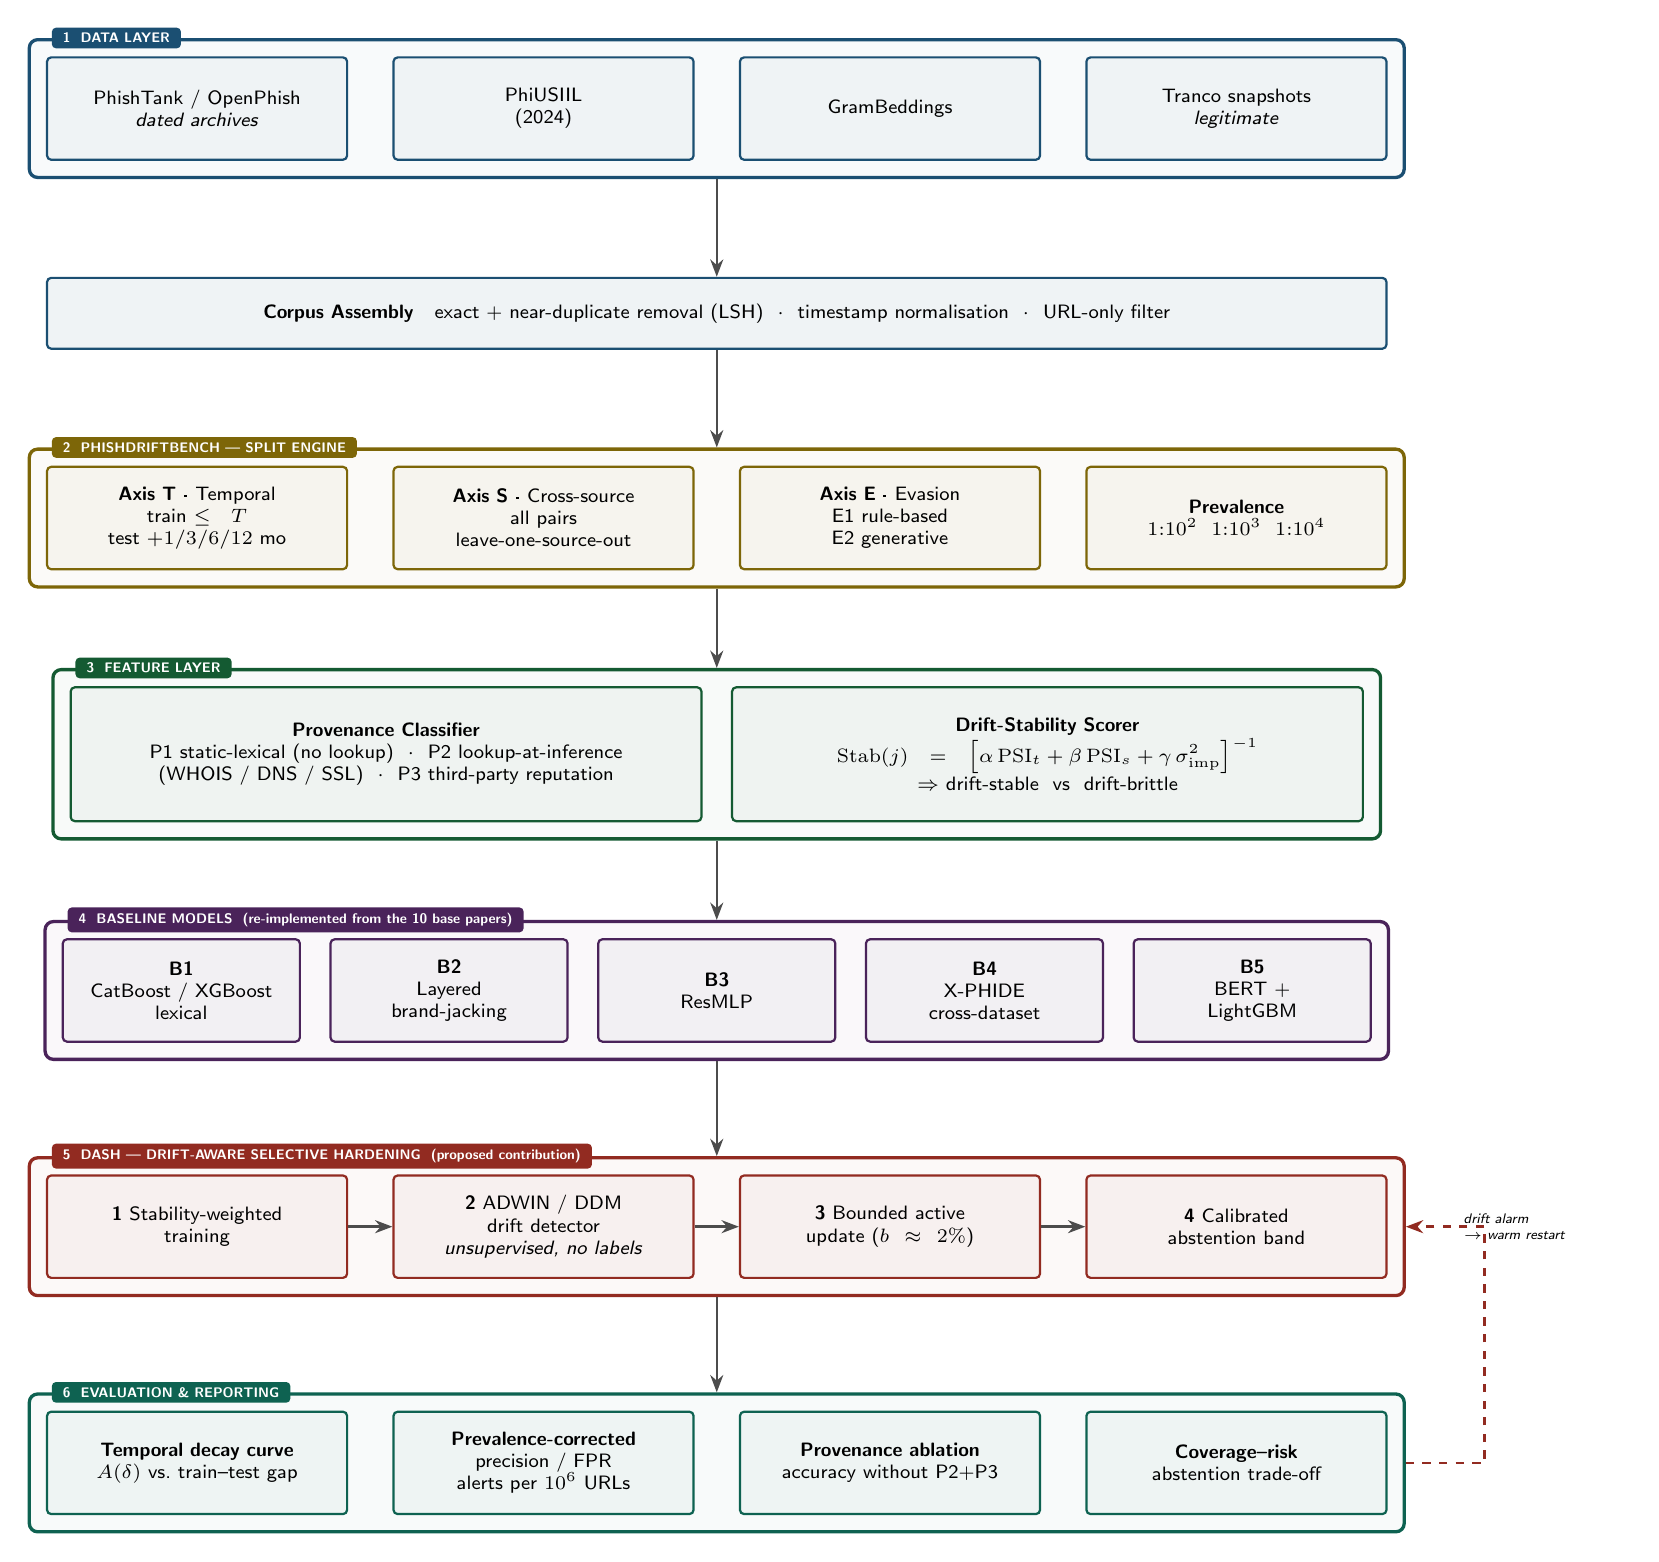
\begin{tikzpicture}[
  x=1mm,y=1mm,font=\scriptsize,
  box/.style 2 args={rectangle,rounded corners=1.5pt,draw=#1,line width=0.8pt,fill=#1!7,
              align=center,inner sep=3pt,minimum height=13mm,text width=#2},
  lay/.style={rectangle,rounded corners=3pt,draw=#1,line width=1.2pt,fill=#1!3,inner sep=6pt},
  lbl/.style={fill=#1,text=white,rounded corners=1.5pt,inner xsep=4pt,inner ysep=2pt,
              font=\bfseries\tiny},
  ar/.style={-{Stealth[length=2.2mm]},line width=0.9pt,draw=black!70}
]

%======================= LAYER 1 : DATA  (y = 0) =======================
\node[box={cData}{36mm}] (d1) at (20,0)  {PhishTank / OpenPhish\\\textit{dated archives}};
\node[box={cData}{36mm}] (d2) at (64,0)  {PhiUSIIL\\(2024)};
\node[box={cData}{36mm}] (d3) at (108,0) {GramBeddings};
\node[box={cData}{36mm}] (d4) at (152,0) {Tranco snapshots\\\textit{legitimate}};
\begin{scope}[on background layer]
  \node[lay=cData,fit=(d1)(d4)] (LD) {};
\end{scope}
\node[lbl=cData,anchor=west] at ($(LD.north west)+(3,0)$) {1 \ DATA LAYER};

%======================= ASSEMBLY (y = -26) =======================
\node[box={cData}{168mm},minimum height=9mm] (asm) at (86,-26)
  {\textbf{Corpus Assembly} \ \ exact + near-duplicate removal (LSH) \ $\cdot$ \ timestamp normalisation \ $\cdot$ \ URL-only filter};
\draw[ar] (LD.south) -- (asm.north);

%======================= LAYER 2 : SPLIT (y = -52) =======================
\node[box={cSplit}{36mm}] (t1) at (20,-52)
  {\textbf{Axis T} · Temporal\\train $\le T$\\test $+1/3/6/12$ mo};
\node[box={cSplit}{36mm}] (t2) at (64,-52)
  {\textbf{Axis S} · Cross-source\\all pairs\\leave-one-source-out};
\node[box={cSplit}{36mm}] (t3) at (108,-52)
  {\textbf{Axis E} · Evasion\\E1 rule-based\\E2 generative};
\node[box={cSplit}{36mm}] (t4) at (152,-52)
  {\textbf{Prevalence}\\$1{:}10^{2}$ \ $1{:}10^{3}$ \ $1{:}10^{4}$};
\begin{scope}[on background layer]
  \node[lay=cSplit,fit=(t1)(t4)] (LS) {};
\end{scope}
\node[lbl=cSplit,anchor=west] at ($(LS.north west)+(3,0)$) {2 \ PHISHDRIFTBENCH — SPLIT ENGINE};
\draw[ar] (asm.south) -- (LS.north);

%======================= LAYER 3 : FEATURE (y = -82) =======================
\node[box={cFeat}{78mm},minimum height=17mm] (pv) at (44,-82)
  {\textbf{Provenance Classifier}\\P1 static-lexical (no lookup) \ $\cdot$ \ P2 lookup-at-inference\\(WHOIS / DNS / SSL) \ $\cdot$ \ P3 third-party reputation};
\node[box={cFeat}{78mm},minimum height=17mm] (st) at (128,-82)
  {\textbf{Drift-Stability Scorer}\\$\mathrm{Stab}(j)=\left[\alpha\,\mathrm{PSI}_{t}+\beta\,\mathrm{PSI}_{s}+\gamma\,\sigma^{2}_{\mathrm{imp}}\right]^{-1}$\\$\Rightarrow$ drift-stable \ vs \ drift-brittle};
\begin{scope}[on background layer]
  \node[lay=cFeat,fit=(pv)(st)] (LF) {};
\end{scope}
\node[lbl=cFeat,anchor=west] at ($(LF.north west)+(3,0)$) {3 \ FEATURE LAYER};
\draw[ar] (LS.south) -- (LF.north);

%======================= LAYER 4 : MODELS (y = -112) =======================
\node[box={cModel}{28mm}] (b1) at (18,-112)  {\textbf{B1}\\CatBoost / XGBoost\\lexical};
\node[box={cModel}{28mm}] (b2) at (52,-112)  {\textbf{B2}\\Layered\\brand-jacking};
\node[box={cModel}{28mm}] (b3) at (86,-112)  {\textbf{B3}\\ResMLP};
\node[box={cModel}{28mm}] (b4) at (120,-112) {\textbf{B4}\\X-PHIDE\\cross-dataset};
\node[box={cModel}{28mm}] (b5) at (154,-112) {\textbf{B5}\\BERT +\\LightGBM};
\begin{scope}[on background layer]
  \node[lay=cModel,fit=(b1)(b5)] (LM) {};
\end{scope}
\node[lbl=cModel,anchor=west] at ($(LM.north west)+(3,0)$)
  {4 \ BASELINE MODELS \ (re-implemented from the 10 base papers)};
\draw[ar] (LF.south) -- (LM.north);

%======================= LAYER 5 : DASH (y = -142) =======================
\node[box={cDash}{36mm}] (h1) at (20,-142)  {\textbf{1} Stability-weighted\\training};
\node[box={cDash}{36mm}] (h2) at (64,-142)  {\textbf{2} ADWIN / DDM\\drift detector\\\textit{unsupervised, no labels}};
\node[box={cDash}{36mm}] (h3) at (108,-142) {\textbf{3} Bounded active\\update ($b\approx2\%$)};
\node[box={cDash}{36mm}] (h4) at (152,-142) {\textbf{4} Calibrated\\abstention band};
\begin{scope}[on background layer]
  \node[lay=cDash,fit=(h1)(h4)] (LH) {};
\end{scope}
\node[lbl=cDash,anchor=west] at ($(LH.north west)+(3,0)$)
  {5 \ DASH — DRIFT-AWARE SELECTIVE HARDENING \ (\textit{proposed contribution})};
\draw[ar] (LM.south) -- (LH.north);
\draw[ar] (h1) -- (h2);
\draw[ar] (h2) -- (h3);
\draw[ar] (h3) -- (h4);

%======================= LAYER 6 : EVAL (y = -172) =======================
\node[box={cEval}{36mm}] (e1) at (20,-172)  {\textbf{Temporal decay curve}\\$A(\delta)$ vs.\ train--test gap};
\node[box={cEval}{36mm}] (e2) at (64,-172)  {\textbf{Prevalence-corrected}\\precision / FPR\\alerts per $10^{6}$ URLs};
\node[box={cEval}{36mm}] (e3) at (108,-172) {\textbf{Provenance ablation}\\accuracy without P2+P3};
\node[box={cEval}{36mm}] (e4) at (152,-172) {\textbf{Coverage--risk}\\abstention trade-off};
\begin{scope}[on background layer]
  \node[lay=cEval,fit=(e1)(e4)] (LE) {};
\end{scope}
\node[lbl=cEval,anchor=west] at ($(LE.north west)+(3,0)$) {6 \ EVALUATION \& REPORTING};
\draw[ar] (LH.south) -- (LE.north);

%======================= FEEDBACK LOOP =======================
\draw[ar,dashed,draw=cDash,line width=1pt]
  (LE.east) -- ++(10,0) -- ++(0,30) -- (LH.east)
  node[midway,right,font=\tiny\itshape,text width=20mm,align=left,xshift=1mm]
  {drift alarm\\$\rightarrow$ warm restart};

\end{tikzpicture}
\end{document}
